
\documentclass{beamer}
\usetheme{metropolis}
\begin{document}
\title{NEAT and HyperNEAT}
\author{Michal Pospěch \& Daniel Crha}
\date{\today}
\institute{Faculty of Mathematics and Physics, Charles University}

\maketitle
\section{Neuroevolution}
\begin{frame}{Fixed Topology Evolution}
    \begin{itemize}
        \item Searching the space of connection weights
        \item Topology is given, does not change during evolution
    \end{itemize}

\end{frame}
\begin{frame}{Evolving Topology}
    \begin{itemize}
        \item Technical challenges:
              \begin{itemize}
                  \item good representation
                  \item not removing non-optimized network to early
                  \item minimisation of networks without need for a complexity function
              \end{itemize}
        \item TWEANNs - Topology and Weight Evolving Artificial Neural Networks
    \end{itemize}

\end{frame}
\section{NEAT}
\begin{frame}{NEAT}
    \begin{itemize}
        \item NeuroEvolution of Augmenting Topologies
        \item Stanley and Miikkulainen, 2002
        \item solves all the issues aforementioned issues
    \end{itemize}
\end{frame}
\begin{frame}{Encoding and Mutation}
    \begin{columns}
        \begin{column}{0.5\textwidth}
            \begin{itemize}
                \item  linear representations of network connectivity
                      \begin{itemize}
                          \item 2 types of genes (nodes and connections)
                          \item innovation number
                          \item node
                      \end{itemize}
                \item 3 types of mutation
                      \begin{itemize}
                          \item connection weight mutation
                          \item new node
                          \item new connection
                      \end{itemize}
            \end{itemize}
        \end{column}
        \begin{column}{0.5\textwidth}
            \begin{figure}[c]
                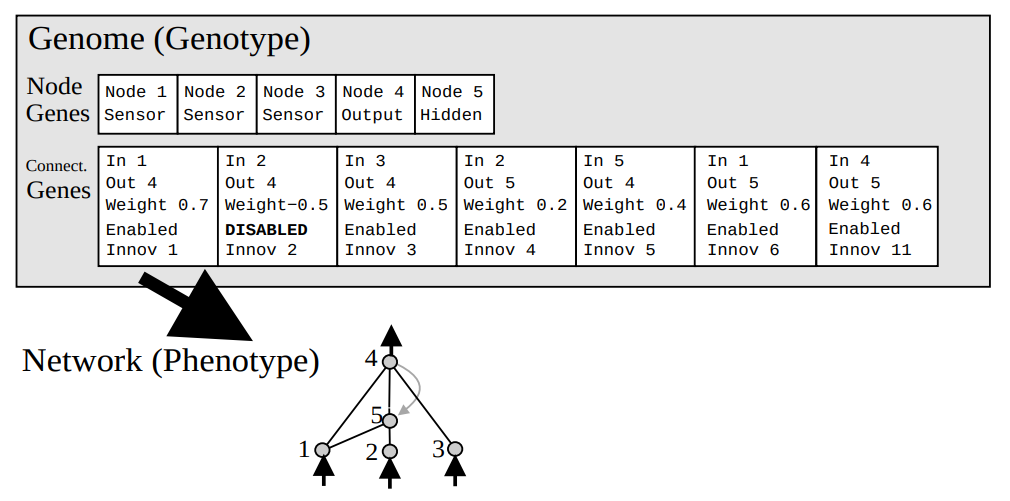
\includegraphics[width = \textwidth]{img/encoding.png}
            \end{figure}
            \begin{figure}[c]
                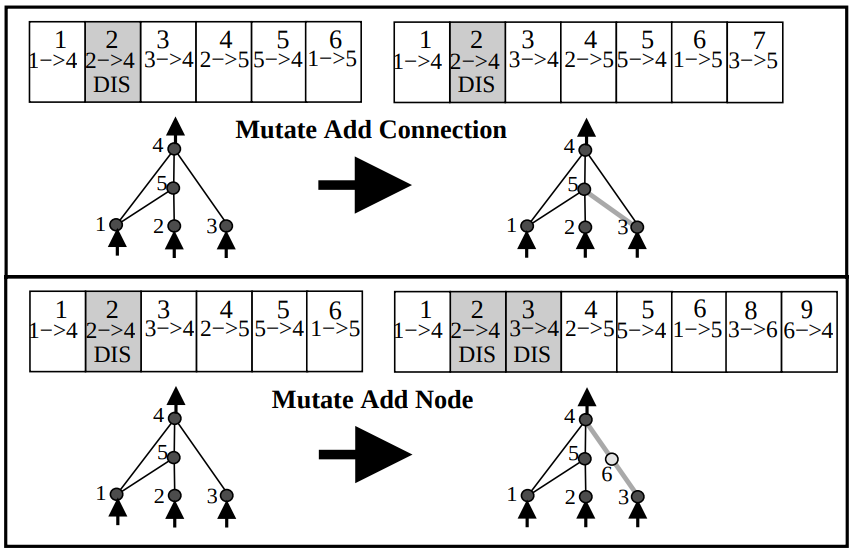
\includegraphics[width = \textwidth]{img/mutation.png}
            \end{figure}
        \end{column}
    \end{columns}
\end{frame}
\begin{frame}{Historical Markings and Crossover}
    \begin{columns}
        \begin{column}{0.7\textwidth}
            \begin{itemize}
                \item innovation number
                      \begin{itemize}
                          \item new node via mutation \textrightarrow global innovation number++
                          \item used to line-up genomes during crossover
                      \end{itemize}
                \item crossover
                \begin{itemize}
                    \item 
                \end{itemize}
                
            \end{itemize}
        \end{column}
        \begin{column}{0.3\textwidth}
           
        \end{column}
    \end{columns}
\end{frame}
\section{HyperNEAT}
\begin{frame}{HyperNEAT}
    \begin{columns}
        \begin{column}{0.5\textwidth}
            some text here some text here some text here some text here some text here
        \end{column}
        \begin{column}{0.5\textwidth}  %%<--- here
            some text here some
        \end{column}
    \end{columns}
\end{frame}
\end{document}
